\section{Time box 3}
\subsection{Time box planning}
Overview of the what work is put into which time boxes.
\begin{figure}[H]
	\begin{centering}
		 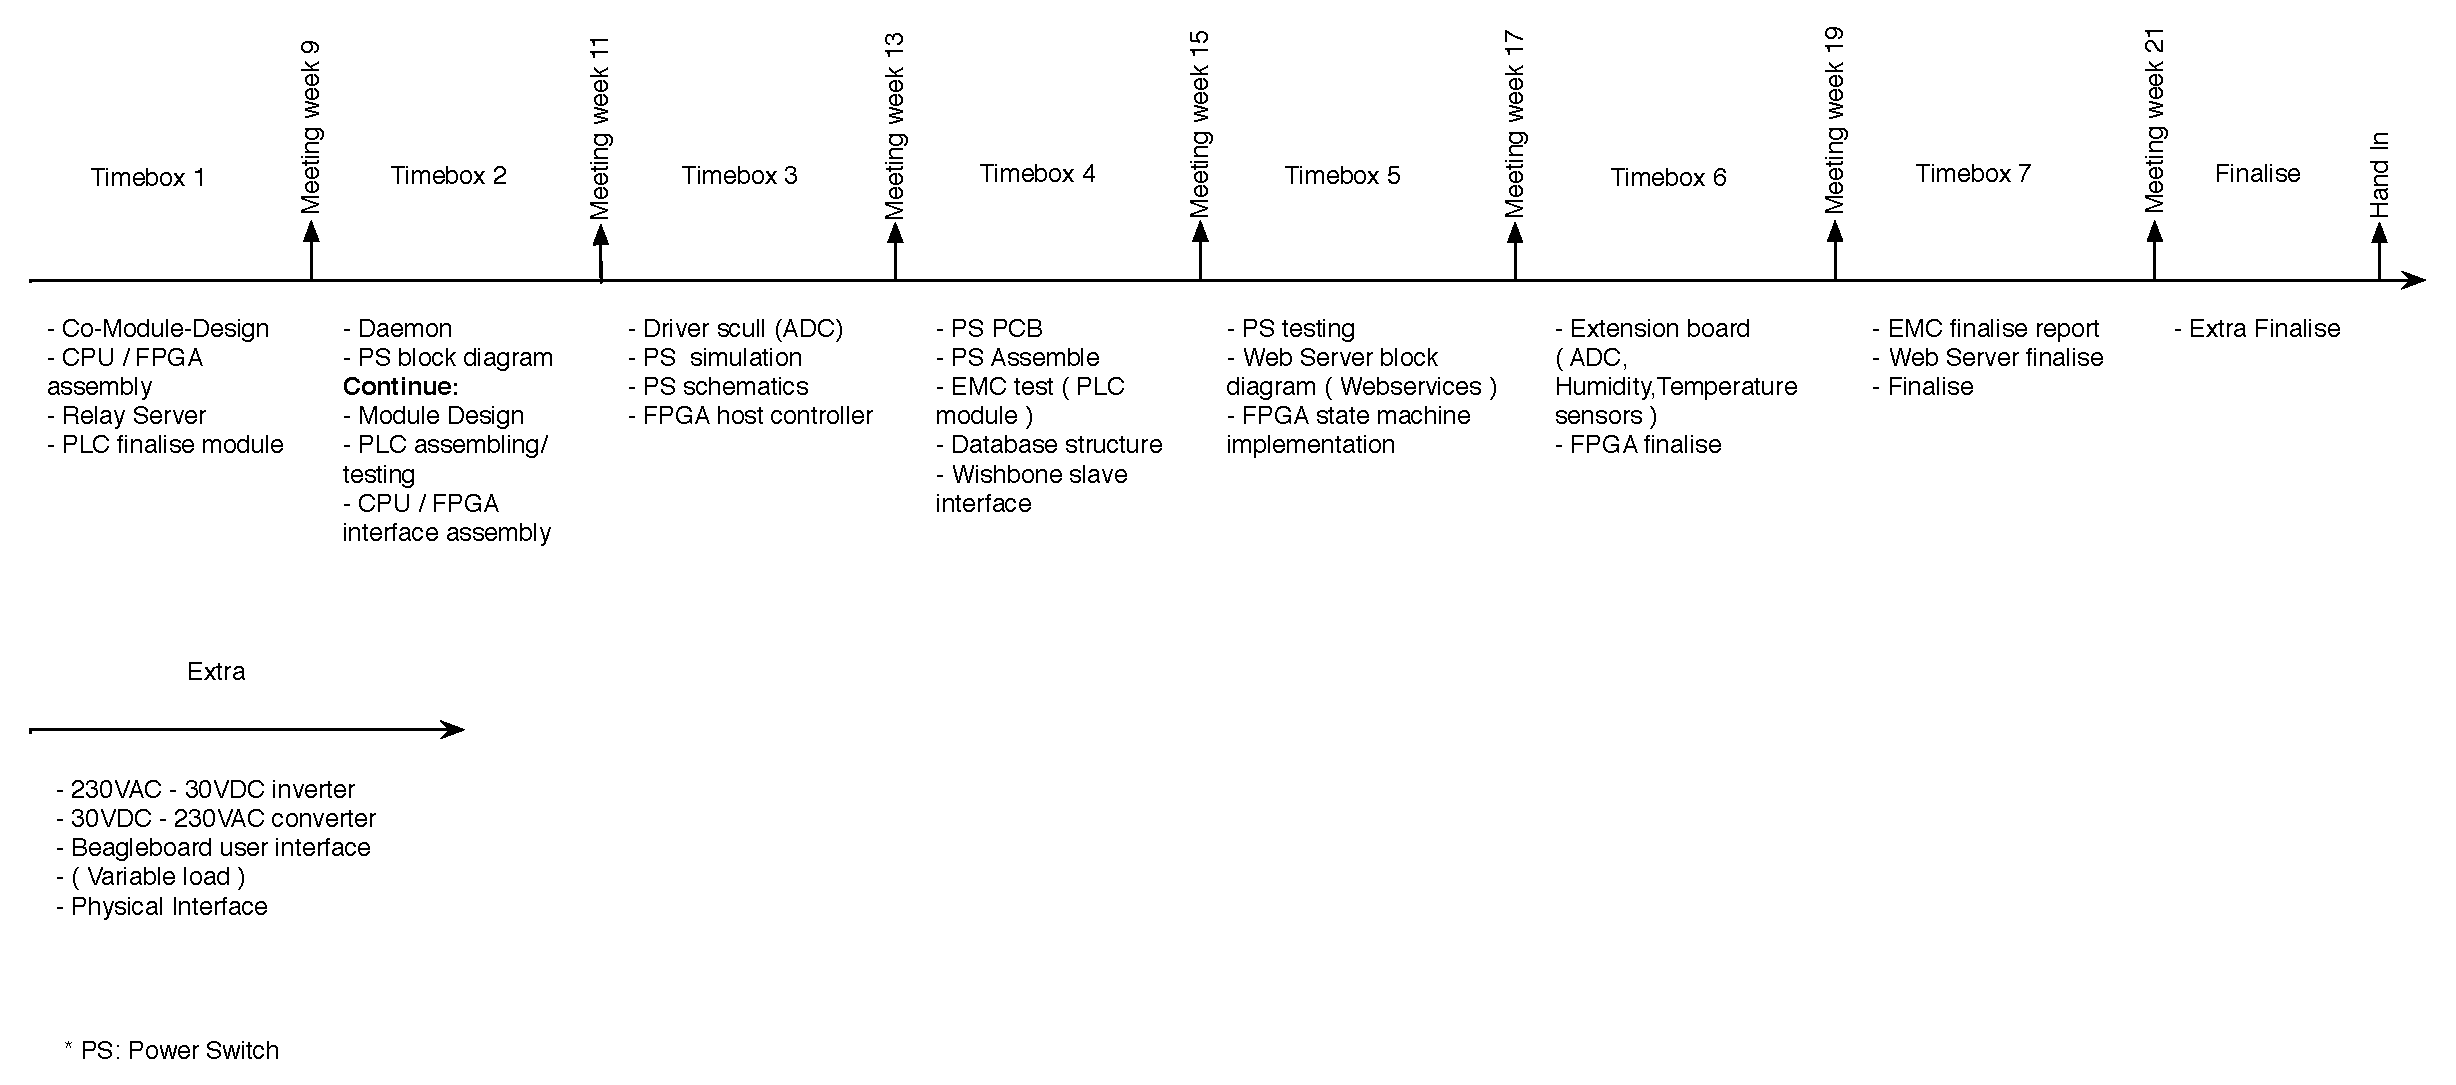
\includegraphics[width=1.0\textwidth]{images/tb_r3.pdf}
		\caption{Updated time-box}
	\end{centering}
\end{figure}

\subsubsection{Work to be done in this time box}
\begin{itemize}
	\item Power switch
	\begin{itemize}
		\item Schematic
		\item Printed circuit board
		\item Mount component
		\item Test board
	\end{itemize}
	\item Host controller
	\begin{itemize}
		\item Master wishbone
		\item CPU interface
	\end{itemize}
\end{itemize}
\paragraph{Description:}
\begin{description}
	\item[Power switch] A single switch port board for the power switch is made, as an essential part for the power switch.
	\item[Host controller] is made in the FPGA, and is responsible for the communication between the Spartan6 and the ARM7, it shall be made with wishbone master interface 
\end{description}

\subsection{Power switch}
\begin{itemize}
	\item Schematic
	\item Printed circuit board
	\item Mount component
	\item Test board
\end{itemize}



\subsection{Host controller}
